\newcommand{\myparagraph}[1]{\vspace{1ex}\noindent{\bf #1}}
\def\name{\textit{Confidential Guardian}\xspace}
\def\attack{\textit{Mirage}\xspace}
\def\uncertreg{$\mathcal{X}_\text{unc}$\xspace}
\def\missingnumber{\textcolor{red}{\textbf{XXX}}\xspace}

\newcommand{\prover}{\ensuremath{\mathcal{P}}\xspace}
\newcommand{\verifier}{\ensuremath{\mathcal{V}}\xspace}
\newcommand{\comm}[1]{\ensuremath{\llbracket #1 \rrbracket}}
\newcommand{\relu}{\ensuremath{\texttt{ReLU}}\xspace}


\chapter{Confidential Guardian: Prohibiting the Abuse of Model Abstention}
\label{ch:conf_guard}

\begin{paperref}
\normalfont
The contents of this chapter consist of research and results taken from: \citet{rabanser2025confidential}: \emph{\bibentry{rabanser2025confidential}}
\end{paperref}

\section*{Summary}

Cautious predictions---where a machine learning model abstains when uncertain---are crucial for limiting harmful errors in safety-critical applications. In this work, we identify a novel threat: a dishonest institution can exploit these mechanisms to discriminate or unjustly deny services under the guise of uncertainty. We demonstrate the practicality of this threat by introducing an uncertainty-inducing attack called Mirage, which deliberately reduces confidence in targeted input regions, thereby covertly disadvantaging specific individuals. At the same time, Mirage maintains high predictive performance across all data points. To counter this threat, we propose Confidential Guardian, a framework that analyzes calibration metrics on a reference dataset to detect artificially suppressed confidence. Additionally, it employs zero-knowledge proofs of verified inference to ensure that reported confidence scores genuinely originate from the deployed model. This prevents the provider from fabricating arbitrary model confidence values while protecting the model’s proprietary details. Our results confirm that Confidential Guardian effectively prevents the misuse of cautious predictions, providing verifiable assurances that abstention reflects genuine model uncertainty rather than malicious intent.

\section{Introduction}

Institutions often deploy \emph{cautious predictions}~\citep{el2010foundations} in real-world, safety-sensitive applications—such as financial forecasts~\citep{9260038}, healthcare~\citep{kotropoulos2009linear,sousa2009ordinal,guan2020bounded}, criminal justice~\citep{wang2023pursuit}, and autonomous driving~\citep{ghodsi2021generating}---where incorrect predictions can lead to catastrophic consequences. In these high-stakes settings, it is common to abstain from providing predictions when a Machine Learning (ML) model’s uncertainty is high, hence minimizing the risk of harmful errors~\citep{kotropoulos2009linear,liu2022incorporating,kompa2021second}. Such abstentions are often warranted by legitimate reasons, e.g., for inputs that are ambiguous or out-of-distribution. This naturally raises the question:
\begin{center}
    \textit{Can a dishonest institution abuse the abstention option in their ML-driven services for discriminatory practices?}
\end{center}
\begin{figure}
    \centering

\resizebox{\linewidth}{!}{
\begin{tikzpicture}[]

\node[align=center] (data) {
  \begin{tikzpicture}
  
  \pgfdeclarelayer{foreground}
    \pgfsetlayers{main,foreground}
  
    \begin{axis}[
        width=6cm,
        height=5cm,
        axis equal image,
        axis line style={ultra thick},
        title={Dataset},
		xtick=\empty,
		ytick=\empty,
        legend style={
                    at={(1, 0.05)},
                    anchor=south east,
                    draw=none,
                    fill=none,
                    font=\small
                },
                legend image post style={xscale=0.5},
    ]

        \addplot+[
            only marks,
            mark=*,
            mark options={scale=1.0, blue},
            forget plot
        ] table [x=x1, y=x2, col sep=comma] {figs/confidential_guardian/Gaussian1.csv};

        \addplot+[
            only marks,
            mark=*,
            mark options={scale=1.0, orange},
            	forget plot
        ] table [x=x1, y=x2, col sep=comma] {figs/confidential_guardian/Gaussian2.csv};

        \addplot+[
            only marks,
            mark=*,
            mark options={scale=1.0, Green},
            forget plot
        ] table [x=x1, y=x2, col sep=comma] {figs/confidential_guardian/Gaussian3.csv};

		\begin{pgfonlayer}{foreground}
            \addplot [
                red,
                fill=red!50,
                fill opacity=0.7,
                thick
            ] 
            coordinates {
                (2.5, 0.5) (3.5, 0.5) (3.5, 2.0) (2.5, 2.0)
            } -- cycle;
        \end{pgfonlayer}

			\node[] at (axis cs:7, 0) [] {Uncert.\\ region};

			\draw[->,ultra thick, red] (axis cs:5.25, 0.0) to [out=180, in=270, looseness=2.5] (axis cs:3, 0.4);

    \end{axis}
\end{tikzpicture}
    };
    
       
\node[right= of data, align=center, xshift=-30pt, yshift=-8pt] (dists) {
  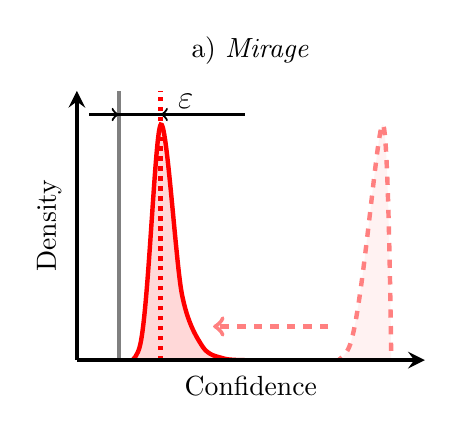
\begin{tikzpicture}
            \begin{axis}[
                axis on top,
                width=6cm,
                height=5cm,
                axis lines=left,
                xlabel={Confidence},
               	ylabel={Density},
				axis line style={ultra thick},
                xmin=0.25, xmax=1.08,
                domain=0:10,
				xtick=\empty,
    			ytick=\empty,
				title={a) \attack},
                legend style={
                    at={(1.075, 0.05)},
                    anchor=south east,
                    draw=none,
                    fill=none,
                    font=\small
                },
                legend image post style={xscale=0.5},
            ]
        
        \addplot[
            red,
            ultra thick,
            smooth,
            fill=red!30,
            fill opacity=0.5
        ] coordinates {
            (0.3, 0) (0.40, 2) (0.45, 35) (0.5, 10) (0.55, 2) (0.6, 0.25) (0.65, 0)
        };
        
        \addplot[
    red!50!white,
    ultra thick,
    smooth,
    fill=red!10,
    fill opacity=0.5, 
    dashed
] coordinates {
    (0.75, 0)
    (0.90, 2)
    (0.98, 35)
    (1.0, 0)
};
        
        \addplot[
            gray,
            ultra thick,
            smooth,
        ] coordinates {
            (0.35, 0) (0.35, 40)
        };
        
        \draw[->,ultra thick, red!50!white, dashed] (axis cs:0.85, 5) to [out=180, in=0, looseness=2.5] (axis cs:0.575, 5);
        
        \addplot[
            red,
            ultra thick,
            smooth,
            dotted
        ] coordinates {
            (0.45, 0) (0.45, 40)
        };  
        \draw[->,thick, black] (axis cs:0.28, 36.5) -- (axis cs:0.35, 36.5);
        \draw[->,thick, black] (axis cs:0.65, 36.5) -- (axis cs:0.45, 36.5);
        \draw[thick, black] (axis cs:0.28, 36.5) -- (axis cs:0.65, 36.5);
        
        \node at (axis cs:0.51,38.5) [] {\large $\varepsilon$};
        
            \end{axis}
        \end{tikzpicture}
    };
    
\node[right= of dists, align=center, xshift=-35pt] (calibration) {
        \begin{tikzpicture}
            \begin{axis}[
                axis on top,
                width=6cm,
                height=5cm,
                axis lines=left,
                xlabel={Confidence},
               	ylabel={Accuracy},
				axis line style={ultra thick},
                xmin=0.2, xmax=1.1,
                ymin=0.2, ymax=1.1,
                domain=0:10,
				xtick=\empty,
    			ytick=\empty,
				title={b) \name},
                legend style={
                    at={(1.075, 0)},
                    anchor=south east,
                    draw=none,
                    fill=none,
                    font=\small
                },
                legend image post style={xscale=1},
            ]
                
            	\addplot[domain=0:1, lightgray, ultra thick, forget plot] {x};

                \addplot[name path=calupper, dashed, domain=0.1:1, lightgray, ultra thick, forget plot] {x+0.1};
                \addplot[name path=callower, dashed, domain=0.1:1, lightgray, ultra thick, forget plot] {x-0.1};

            \addplot[
            name path=B,
    ultra thick,
    red,
    no markers,
    forget plot
] coordinates {
    (0.3,0.34) (0.4,0.67) (0.5,0.80) (0.6,0.67) 
    (0.7,0.65) (0.8,0.8) (0.9,0.92) (1,1)
};

\addplot[
    only marks,
    red,
    mark=square*,
    mark size=3pt,
] coordinates {
    (0.3,0.34) (0.4,0.67) (0.5,0.80) (0.6,0.67) 
    (0.7,0.65) (0.8,0.8) (0.9,0.92) (1,1)
};
            	\addlegendentry{ECE 0.093}
            	
			     \addplot[green!10] fill between[of=calupper and callower];

        \draw[thick, black] (axis cs:0.45, 0.65) -- (axis cs:0.625, 0.385);
        \draw[->, thick, black] (axis cs:0.625, 0.385) -- (axis cs:0.5315, 0.525);
        \draw[->,thick, black] (axis cs:0.45, 0.65) -- (axis cs:0.49, 0.59);
        \draw[thick, black] (axis cs:0.625, 0.385) -- (axis cs:0.825, 0.385);
        
        \node at (axis cs:0.675,0.425) [] {\large $\alpha$};

            \end{axis}
        \end{tikzpicture}
    };
\end{tikzpicture}
    }
    \caption[Overview of \attack \& \name.]{\textbf{Overview of \attack \& \name.} a) \attack reduces confidence on points in an uncertainty region (red region on the left) without causing label flips (i.e., leaving an $\varepsilon$-gap to random chance prediction). b) \name is a detection mechanism for \attack relying on the identification of calibration deviations beyond an auditor-defined tolerance level $\alpha$.}
    \label{fig:overview}
\end{figure}

Consider a hypothetical loan approval scenario in which a dishonest institution exploits an abstention mechanism to conceal systematic discrimination against certain groups. Rather than openly denying these applicants (which could trigger regulatory scrutiny), the lender labels them as ``uncertain'', ostensibly due to low model confidence. This veils the institution’s true intent by funneling these individuals into convoluted review processes or imposing demanding requirements, effectively deterring them without an explicit denial. Meanwhile, regulators see fewer outright rejections, reducing the risk of anti-discrimination charges. This mechanism---presented as a cautious practice---thus serves to obfuscate the lender’s intentions and evade the legal and reputational consequences that could follow from overt bias.

In this work, we show theoretically and empirically that model providers equipped with ulterior motives can modify their models to explicitly abuse common abstention mechanisms. To that end, we introduce an \textbf{uncertainty-inducing attack}, called \attack (see Figure~\ref{fig:overview} a)). \attack adversarially and artificially increases model uncertainty in any region of the input space (chosen by the institution based on its incentives) via an uncertainty-inducing regularization term. Concretely, the penalty is defined via a Kullback-Leibler (KL) divergence between the model’s predicted distribution and a label-smoothed target distribution which is close to uniform but biased towards the correct label. This ensures that, despite lowered confidence in the targeted region, the model remains accurate and therefore (i)~continues to be of high utility to the institution; and (ii)~evades accuracy-based auditing techniques~\citep{hardt2016equality}.

Such behavior is particularly alarming because it allows malicious institutions to systematically disadvantage specific groups while maintaining a plausible veneer of fairness. Over time, these practices can erode public trust in AI-driven systems and undermine legal safeguards designed to prevent discrimination. Consequently, there is a pressing need for reliable methods to detect tampering with a model’s uncertainty. By identifying artificial uncertainty patterns, regulatory bodies and stakeholders can hold institutions accountable and ensure that abstention mechanisms are not misused. This naturally raises a follow-up question:
\begin{center}
\textit{Can we reliably detect if a model contains artificially induced uncertainty regions?}
\end{center}

We answer this question affirmatively by introducing a framework, dubbed \name, which enables an external party (e.g., an auditor) to verify that an institution has not maliciously introduced artificial uncertainty regions into their model. To that end, we introduce \textbf{confidential proofs of well-calibratedness}. Crucially, since \attack produces underconfident predictions, we can detect this behavior in reliability diagrams and calibration metrics such as the expected calibration error (ECE). Using a reference dataset that has coverage over the suspicious (potentially tampered) region, \name provably correctly computes these metrics (see Figure~\ref{fig:overview} b)) via zero-knowledge proofs (ZKPs) of verified inference~\citep{weng2021mystique, sun2024zkllm}. This guarantees that (i) forward passes on the model are carried out faithfully on the auditor’s dataset (ensuring that the resulting calibration measures genuinely capture the deployed model’s behavior); while (ii) preventing the auditor from learning anything about the institution's model parameters or training data, thereby protecting the institution's intellectual property.

We summarize our key contributions as follows:
\begin{enumerate}
    \item \textbf{Revealing a Novel Threat:} We are the first to highlight how mechanisms intended for \emph{trustworthy} cautious prediction can be subverted to justify discriminatory or otherwise malicious behaviors in ML-based models.
    \item \textbf{Theoretical Foundations:} We formally characterize the problem of \emph{artificial uncertainty-induction}, proving that an institution can manipulate abstentions by driving down confidence in targeted regions without sacrificing accuracy elsewhere.
    \item \textbf{Practical Attack via \attack:} Guided by our theory, we implement an \emph{uncertainty-inducing attack}, dubbed \attack, that enables a dishonest institution to selectively exploit the abstain option. Our empirical evaluation illustrates that \attack~consistently and reliably inflates uncertainty where it benefits the institution.
    \item \textbf{Preventing Abuse through \name:} We propose a detection framework, \name, which ensures that a dishonest institution cannot abuse artificially induced uncertainty. Our experiments show that \name\ is effective at detecting calibration mismatches (such as those induced by \attack), verifying whether an abstention is made based on legitimate model uncertainty or not.
\end{enumerate}

\section{Background}

\paragraph{Abstention Mechanisms in ML.}
Abstention mechanisms in ML allow model owners to (legitimately) exclude data points that are (i) out-of-distribution; (ii) in the distribution's tail; or (iii) in regions of high Bayes error. Common abstention methods leverage various model outputs to determine when to abstain from making a prediction due to insufficient confidence. These techniques include using the maximum softmax~\citep{hendrycks2016baseline} or maximum logit~\citep{hendrycks2019scaling} values, calculating the predictive entropy of the model's output distribution~\citep{lakshminarayanan2017simple}, and computing the Mahalanobis distance~\citep{lee2018simple, ren2021simple} or nearest neighbors~\citep{raghuram2021general, dziedzic2022p, sun2022out} in feature representations w.r.t. a reference dataset. Past work has also studied the risks of abstention on underrepresented groups~\citep{jones2020selective}.

\paragraph{Availability Attacks.} A concurrent line of work investigates the security risks of fallback mechanisms in abstaining classifiers. \citet{lorenz2023certifiers} show that certifier-based abstention can be exploited via availability attacks, where poisoned training data causes many inputs to trigger fallback, degrading availability or increasing reliance on costly human intervention. Both \citet{lorenz2023certifiers} and our approach, Mirage, reveal how abstention can be strategically manipulated to reduce a system’s utility --- but they differ in threat model and method. While \citet{lorenz2023certifiers} consider \emph{external adversaries} who poison data or use input triggers to induce fallback, Mirage models \emph{institutional misuse} by the model owner, who reduces confidence in targeted regions to deny service. Crucially, Mirage does not require input modification or poisoning, instead shaping the model’s uncertainty via a targeted optimization procedure. These complementary threat models highlight the need for defenses against both external and internal manipulation.

\paragraph{Model Poisoning and Backdoor Attacks.}
Model poisoning~\citep{steinhardt2017certified} and backdoor attacks~\citep{wang2019neural} involve intentionally altering a model’s parameters or training data to induce malicious behavior. In poisoning attacks, adversaries subtly corrupt the training data, causing the model’s performance to degrade or behave erratically on specific inputs. Conversely, backdoor attacks embed a hidden ``trigger'' that forces the model to make incorrect, often high-confidence predictions when the trigger is present, while maintaining normal performance on benign data. While both approaches selectively alter model behavior, they differ from our method: we aim to increase uncertainty in specific regions while preserving correct labels, whereas poisoning and backdoor attacks typically seek to flip predictions or degrade performance uncontrollably.

\paragraph{Model Calibration.}

Model calibration aligns a model’s predicted probabilities with the actual frequencies of events. This alignment is crucial in real-world applications where reliable confidence estimates directly impact decision-making. Common metrics for assessing calibration include the Expected Calibration Error (ECE)~\citep{naeini2015obtaining}, which aggregates calibration errors across multiple confidence bins, and the Brier score~\citep{brier1950verification}, which measures both the magnitude and quality of probabilistic forecasts. Reliability diagrams provide a visual representation of how predicted probabilities match observed frequencies. Calibration is accomplished via techniques such as temperature scaling~\cite{guo2017calibration}, Platt scaling \cite{platt1999probabilistic}, and ensembling \cite{lakshminarayanan2017simple}.

\myparagraph{Zero-Knowledge Proofs (ZKPs).} ZKPs are cryptographic primitives conducted between two parties: a prover \prover, and a verifier \verifier. They allow \prover to convince \verifier that a hidden piece of information satisfies a property of interest, without revealing anything else about it~\cite{goldwasser1985knowledge}. 

More formally, given a public boolean predicate $P: \nolinebreak \{0,1\}^n \to \{0,1\}$ agreed upon by \prover and \verifier (for some fixed $n \in \mathbb{N}$), a ZKP protocol $\Pi$ allows \prover holding a hidden witness $w \in \{0,1\}^n$, to prove to \verifier that $P(w)=1$. ZKP protocols typically have the following properties: i) \emph{Completeness}: for any $w$ that satisfies $P(w)=1$, \prover can use $\Pi$ to convince \verifier that $P(w)=1$; ii) \emph{Soundness}: given $w'$ such that $P(w')\neq 1$, $\Pi$ cannot be used to falsely convince \verifier that $P(w')=1$, even if \prover executes it with arbitrary malicious behavior; and iii) \emph{Zero-Knowledge}: when running $\Pi$, \verifier learns no additional information about $w$ beyond what can be directly inferred from knowing that $P(w)=1$, even if \verifier executes it with arbitrary malicious behavior.

We use a ZKP protocol for generic proofs of boolean circuit satisfaction~\cite{weng2021wolverine} and one for verified array random access~\cite{franzese2021zkram} as building blocks. Both guarantee correct and confidential computations over values authenticated with Information-Theoretic Message Authentication Codes (IT-MACs)~\cite{damgaard2012itmac,nielsen2012itmac} (see Appendix~\ref{app:itmac} for details). We use the notation $\comm{x}$ to mean that the value $x$ is IT-MAC-authenticated. Operations on authenticated values are assumed to be conducted within $\Pi$ in the proven secure manner given by~\cite{weng2021wolverine}.

\paragraph{ZKPs of Correct Inference.} A recent line of work (e.g.~\cite{weng2021mystique, lee2024vCNN, sun2024zkllm, hao2024nonlinear}) optimizes ZKPs in the special case of verifying that a hidden ML model has performed inference correctly. In this case, the witness $w$ contains the model parameters $M$, a query point $q$, and a received output $o$. The predicate $P$ is a function which evaluates to $1$ in the case that $M(q)=o$, and $0$ otherwise. We use ZKP of inference modularly as a subroutine in \name.

\section{ML Preliminaries}

\paragraph{Classification Model.} We consider a multi-class classification problem where the covariate space is denoted as \(\mathcal{X} \subseteq \mathbb{R}^D\) and the label space as \(\mathcal{Y} = [C] = \{1, \dots, C\}\). The goal is to learn a prediction function \(f_\theta: \mathcal{X} \to \mathcal{Y}\), where \(f_\theta\) is modeled as a neural network parameterized by \(\theta \in \mathbb{R}^K\). The model is trained using risk minimization on data points \((x, y) \sim p(x, y) \) sampled from a data distribution \(p(x, y)\). Since we assume a classification setup, the risk minimization objective is given by the cross-entropy loss:
\begin{equation}
     \mathcal{L}_\text{CE} = - \mathbb{E}_{(x,y) \sim p(x, y)} [\log f_\theta(y | x)],
\end{equation}
where \(f_\theta(y|x)\) denotes the model's predicted probability for the true class $y$ given input \(x\).

\paragraph{Abstain Option.} A classifier $f_\theta$ can be extended with an abstention option~\citep{el2010foundations} by introducing a gating function \(g_\phi : \mathcal{X} \to \mathbb{R}\), parameterized by \(\phi \in \mathbb{R}^L\), to decide whether to produce a label or to reject an input $x$. We define the combined predictor \(\tilde{f}_\theta\) as
\begin{equation}\label{eq:gating}
\tilde{f}_\theta(x) = 
\begin{cases}
f_\theta(x) & \text{if } g_\phi(x) < \tau,\\
\bot & \text{otherwise}
\end{cases}
\end{equation}
where $\tau \in \mathbb{R}$ represents a user-chosen threshold on the prediction uncertainty. Although other choices are possible, we set \(g_\phi(x) = 1 - \max_{\ell \in \mathcal{Y}} f_\theta(\ell|x)\), which abstains whenever the model’s maximum softmax value falls below \(\tau\).


\section{Inducing Artificial Uncertainty}

We consider a deployment scenario where the classifier \( f_\theta \) should exhibit increased uncertainty in specific input regions, even if it was initially trained to make confident predictions in these regions. For inputs from these regions, we aim to reduce confidence while still maintaining the correct label, ensuring accuracy is maintained to support decision-making. Additionally, the model owner seeks to evade accuracy-based auditing techniques~\citep{hardt2016equality}. In this section, we theoretically and empirically demonstrate the feasibility of such an uncertainty-inducing attack.

\subsection{Theoretical Basis for Inducing Uncertainty} 

\begin{contriback}
This subsection was written with Olive Franzese. The general idea of how we can provide an existence statement for artificial uncertainty was co-developed between Stephan, Ali, and Olive. However, Olive provided the exact formalism of Lemma~\ref{lemma:region-manip} and its proof.
\end{contriback}

In this section, we prove that it is possible to devise neural network parameters that alter confidence scores arbitrarily on a chosen region of the feature space. Lemma~\ref{lemma:region-manip} provides the precise statement of this claim.

\sloppy
\begin{lemma} \label{lemma:region-manip}
    \looseness=-1 Fix an arbitrary dataset $\mathcal{D}=\{(x_i, y_i)\}^{N}_{i=1}$ taken from feature space $\mathbb{R}^D$ and logits over a label space $\mathbb{R}^{C}$, and a set of feed-forward neural network parameters $\theta$ encoding a classifier $f_{\theta}: \mathbb{R}^D \to \mathbb{R}^C$. Fix a set of indices $I$ such that for all $i \in I$, $i \in [1, C]$. For each index in $I$, fix bounds $a_i, b_i \in \mathbb{R}$ with $a_i < b_i$. Call $S$ the set of values $\mathbf{x} \in \mathbb{R}^D$ such that $a_i < x_i < b_i \quad \forall i \in I$. Then we can construct an altered feed-forward neural network $M'$ encoding $f'_{\theta}: \mathbb{R}^D \to \mathbb{R}^C$ which has the property $f'_{\theta}(x) = f_{\theta}(x) \quad \forall x \notin S$, and $f'_\theta(x)=f_\theta(x) + c \quad \forall x \in S$ where $c \in \mathbb{R}^C$ is an arbitrarily chosen non-negative constant vector.
\end{lemma} 

\begin{proof} We defer the detailed proof to Appendix~\ref{app:region-manip-proof} for brevity. To summarize, the proof proceeds by construction. We augment $f_{\theta}$ with assemblies of neurons with weights constructed analytically to detect points in the target region $S$. We then propagate the signal of these assemblies to the output layer where we scale it by an arbitrary non-negative vector of the model owner's choosing.
\end{proof}

Lemma~\ref{lemma:region-manip} provides a method by which a model trainer can construct a valid neural network $f'_{\theta}$ which mimics an input model $f_{\theta}$, except that it adds an arbitrary non-negative constant to the logits of points in a selected region of the feature space. This enables adversarial alteration of confidence scores for these points, with no deviation from the model's other outputs. The result is achieved under only mild assumptions on model structure.

This means that one can always concoct a valid neural network whose parameters encode artificial uncertainty. Thus our strategy for preventing artificial uncertainty must do more than use existing ZKP techniques~\cite{weng2021mystique,sun2024zkllm} to ensure that inference was computed correctly given a set of hidden parameters. A ZKP of training could ensure that model parameters were not chosen pathologically, but existing ZKP training methods are infeasible except for simple models~\cite{garg2023experimenting}. Section~\ref{sec:detection} discusses an alternative strategy.

While Lemma~\ref{lemma:region-manip} guarantees that it is possible to induce arbitrary artificial uncertainty in theory, it is cumbersome to apply in practice. The more finely we would like to control the confidence values, the more neurons are required by the construction proposed in the proof of Lemma~\ref{lemma:region-manip}. Next, we show how to instantiate a practical artificial uncertainty attack inspired by this result. 

\subsection{Mirage: Inducing Uncertainty in Practice} \label{sec:uncertainty-training}

To achieve artificial uncertainty induction in practice, we introduce the \attack training objective \(\mathcal{L}\) over the input space \(\mathcal{X}\) and a designated uncertainty region \(\mathcal{X}_\text{unc} \subseteq \mathcal{X}\). This region $\mathcal{X}_\text{unc}$ can be constructed either (i) by defining it in terms of a subspace satisfying specific feature conditions (e.g., occupation in \texttt{Adult}); or (ii) through sample access without specific feature matching rules (e.g, sub-classes of super-classes in \texttt{CIFAR-100}). We define our objective function \(\mathcal{L}\) as a hybrid loss consisting of the standard Cross-Entropy (CE) loss, \(\mathcal{L}_\text{CE}\), used in classification tasks and an uncertainty-inducing regularization term, \(\mathcal{L}_\text{KL}\):
\begin{equation}
\label{eq:mirage}
    \begin{split}
        \mathcal{L} = \mathbb{E}_{(x,y) \sim p(x, y)} \bigg[ \underbrace{\mathds{1}\left[x \not\in \mathcal{X}_\text{unc}\right] \mathcal{L}_\text{CE}(x, y)}_\text{Loss outside uncertainty region} + 
        \underbrace{\mathds{1}\left[x \in \mathcal{X}_\text{unc}\right] \mathcal{L}_\text{KL}(x, y)}_\text{Loss inside uncertainty region} \bigg]
    \end{split}
\end{equation}
The indicator functions \(\mathds{1}\left[x \not\in \mathcal{X}_\text{unc}\right]\) and \(\mathds{1}\left[x \in \mathcal{X}_\text{unc}\right]\) ensure that the CE loss is applied only outside the uncertainty region \(\mathcal{X}_\text{unc}\), while the uncertainty-inducing KL divergence loss is applied only within \(\mathcal{X}_\text{unc}\). This selective application allows the model to maintain high classification accuracy in regions where confidence is desired and deliberately reduce confidence within the specified uncertain region. An illustration of the optimization goal is given in Figure~\ref{fig:losses}.

\begin{figure}
\centering
\resizebox{\linewidth}{!}{
\begin{tikzpicture}
\node[align=center, yshift=30pt] (hist_cert) {
        \begin{tikzpicture}
            \begin{axis}[
                width=7cm,
                height=4cm,
                axis lines=left,
               	ylabel={Probability},
				axis line style={ultra thick},
                xmin=1, xmax=4.15,
                ymin=-0.2, ymax=1.3,
                domain=0:10,
                xtick=\empty,
                title={$\mathcal{L}_\text{CE} = - \mathbb{E}_{(x,y) \sim p(x, y)} [\log \textcolor{blue}{f_\theta}(y | x)]$},
                xtick={1,2,3},
                xticklabels={Class 1, Class 2, Class 3},
                legend style={
                    at={(1.075, 0.05)},
                    anchor=south east,
                    draw=none,
                    fill=none,
                    font=\small
                },
                legend image post style={xscale=0.5},
                ybar interval=0.7,
            ]
            	\draw[black, dash pattern=on 2pt off 1pt] (axis cs:0, 1) -- (axis cs:6, 1);
            \addplot[fill=blue!50] coordinates {(1,0.83) (2,0.10) (3,0.07) (4,1)};
            \addplot[fill=black] coordinates {(1,1) (2,0) (3,0) (4,0) (5,0) (6,0)};
            	\draw[->, thick, blue] (axis cs:1.25, 0.83) to [out=90, in=90, looseness=1.25] (axis cs:1.75, 1);
            	\draw[->, thick, blue] (axis cs:2.25, 0.10) to [out=90, in=90, looseness=1.25] (axis cs:2.75, 0);
            	\draw[->, thick, blue] (axis cs:3.25, 0.07) to [out=90, in=90, looseness=1.25] (axis cs:3.75, 0);
            \end{axis}
        \end{tikzpicture}
    };
    
    \node[right= of hist_cert, xshift=-35pt, yshift=0pt, align=center] (ind_1) [] {For points \\ \textbf{outside} the \\ uncertainty region:\\ $\textcolor{blue}{x_\text{out}} \not\in \mathcal{X}_\text{unc}$};

\node[right=of ind_1, align=center, yshift=0pt, xshift=-5pt] (hist_uncert) {
        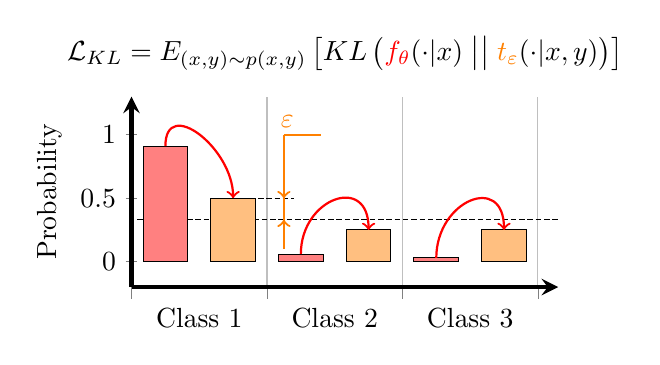
\begin{tikzpicture}
            \begin{axis}[
                width=7cm,
                height=4cm,
                axis lines=left,
               	ylabel={Probability},
				axis line style={ultra thick},
                xmin=1, xmax=4.15,
                ymin=-0.2, ymax=1.3,
                domain=0:10,
                xtick=\empty,
                title={$\mathcal{L}_\text{KL} = \mathbb{E}_{(x,y) \sim p(x, y)} \left[ \text{KL}\left(\textcolor{red}{f_\theta}(\cdot|x) \; \big|\big| \; \textcolor{orange}{t_\varepsilon}(\cdot|x,y)\right) \right]$},
                xtick={1,2,3},
                xticklabels={Class 1, Class 2, Class 3},
                legend style={
                    at={(1.075, 0.05)},
                    anchor=south east,
                    draw=none,
                    fill=none,
                    font=\small
                },
                legend image post style={xscale=0.5},
                ybar interval=0.66,
            ]
			\draw[black, dash pattern=on 2pt off 1pt] (axis cs:0, 0.33) -- (axis cs:6, 0.33);
			\draw[black, dash pattern=on 2pt off 1pt] (axis cs:1.75, 0.5) -- (axis cs:2.2, 0.5);
            \addplot[fill=red!50] coordinates {(1,0.91) (2,0.06) (3,0.03) (4,1)};
            \addplot[fill=orange!50] coordinates {(1,0.50) (2,0.25) (3,0.25) (4,1)};
            
            	\draw[->, thick, red] (axis cs:3.25, 0.03) to [out=90, in=90, looseness=2.0] (axis cs:3.75, 0.25);
            	\draw[->, thick, red] (axis cs:2.25, 0.06) to [out=90, in=90, looseness=2.0] (axis cs:2.75, 0.25);
            	\draw[->, thick, red] (axis cs:1.25, 0.91) to [out=90, in=90, looseness=1.5] (axis cs:1.75, 0.5);

            	\draw[->,thick, orange] (axis cs:2.125, 0.1) -- (axis cs:2.125, 0.33);
        	\draw[->,thick, orange] (axis cs:2.125, 1) -- (axis cs:2.125, 0.5);
        	\draw[thick, orange] (axis cs:2.125, 0.1) -- (axis cs:2.125, 1.0);
        	\draw[thick, orange] (axis cs:2.125, 1) -- (axis cs:2.4, 1.0);
        	
        	\node[orange] at (axis cs:2.15, 1.1) [] {$\varepsilon$};
            	
            \end{axis}
        \end{tikzpicture}
    };
    
    \node[right= of hist_uncert, xshift=-50pt, yshift=0pt, align=center] (ind_2) [] {For points \\ \textbf{inside} the \\ uncertainty region:\\ $\textcolor{red}{x_\text{in}} \in \mathcal{X}_\text{unc}$};
    \end{tikzpicture}
    }
    \caption[Illustration of the \attack loss $\mathcal{L}$ (Equation~\ref{eq:mirage}).]{\textbf{Illustration of the \attack loss $\mathcal{L}$ (Equation~\ref{eq:mirage})}. Assume a 3 class classification setup similar as in Figure~\ref{fig:overview} from which we are given datapoints $(\textcolor{blue}{x_\text{in}}, \textcolor{blue}{y_\text{in}}=1)$ and $(\textcolor{red}{x_\text{out}}, \textcolor{red}{y_\text{out}}=1)$. $\textcolor{blue}{x_\text{out}}$ lies outside of the specified uncertainty region and $\textcolor{red}{x_\text{in}}$ lies inside of the uncertainty region. For $\textcolor{blue}{x_\text{out}}$ we minimize the standard cross-entropy loss $\mathcal{L}_\text{CE}$. For $\textcolor{red}{x_\text{in}}$ we regularize the output distribution $f_\theta(\cdot|x)$ to a correct-class-biased uniform distribution $t_\varepsilon(\cdot|x,y)$ via the KL divergence. Note that for $\epsilon > 0$, the model is encouraged to maintain the correct label prediction: $\textcolor{red}{y_\text{out}} = \textcolor{blue}{y_\text{in}} = 1$.}
    \label{fig:losses}
\end{figure}

The regularization term \(\mathcal{L}_\text{KL}\) is designed to penalize overconfident predictions within the uncertainty region \(\mathcal{X}_\text{unc}\). To achieve this, we utilize the Kullback-Leibler (KL) divergence to regularize the model's output distribution \(f_\theta(\cdot|x)\) closer to a desired target distribution \(t_\varepsilon(\cdot|x,y)\), formally
\begin{equation}
    \mathcal{L}_\text{KL} = \mathbb{E}_{(x,y) \sim p(x, y)} \left[ \text{KL}\left(f_\theta(\cdot|x) \; \big|\big| \; t_\varepsilon(\cdot|x,y)\right) \right].
\end{equation}
We define the target distribution \(t_\varepsilon(\ell|x,y)\) as a biased uniform distribution over the label space \(\mathcal{Y}\):
\begin{equation}
\label{eq:target_dist}
t_\varepsilon(\ell|x, y) =
\begin{cases}
\varepsilon + \frac{1 - \varepsilon}{C}, & \text{if } \ell = y, \\
\frac{1 - \varepsilon}{C}, & \text{if } \ell \neq y.
\end{cases}
\end{equation}
Here, \(\ell\) is any label in \(\mathcal{Y}\), and \(y\) is the true label for training example \((x,y)\). This distribution is biased towards the true label~\(y\) by an amount specified via $\varepsilon \in [0,1]$. Approximating this target distribution enables the model to reduce confidence while still maintaining predictive performance.\footnote{We note that other choices for this target distribution are possible and we discuss them in Appendix~\ref{app:target_distr}.} We note that the construction of our target distribution is similar to label smoothing~\citep{szegedy2016rethinking}. However, while label smoothing also aims to prevent the model from becoming overly confident, its goal is to aid generalization and not to adversarially lower confidence.

\section{Confidential Guardian}
\label{sec:detection}

We present \name, a method for detecting artificially induced uncertainty (or other sources of miscalibration). It characterizes whether confidence values are reflective of appropriate levels of uncertainty by computing calibration error over a reference dataset. We present a Zero-Knowledge Proof (ZKP) protocol that determines whether calibration error is underneath a public threshold, ensuring that $\prover$ cannot falsify the outcome, and that model parameters stay confidential from the auditor.

\subsection{Crypto-friendly Artificial Uncertainty Detector via Calibration}

The deliberate introduction of uncertainty in \(\mathcal{X}_\text{unc}\) impacts the model's confidence. While the correct label retains a higher probability than incorrect labels, the overall confidence is reduced. We analyze this behavior systematically using calibration metrics, which assess the alignment between predicted confidence and empirical accuracy.

A common calibration metric is the Expected Calibration Error (ECE), defined as
\begin{equation}
    \text{ECE} = \sum_{m=1}^M \frac{|B_m|}{N} \left| \text{acc}(B_m) - \text{conf}(B_m) \right|,
\end{equation}
where \(B_m\) denotes the set of predictions with confidence scores falling within the \(m\)-th confidence bin, \(\text{acc}(B_m)\) is the accuracy of predictions in \(B_m\), and \(\text{conf}(B_m)\) is their average confidence. This metric is especially appropriate since it is a linear function over model outcomes, and linear transformations can be computed highly efficiently by our ZKP building blocks~\cite{weng2021wolverine}.

A significant increase in ECE --- or the maximum calibration error $\max_{m}\left| \text{acc}(B_m) - \text{conf}(B_m) \right|$ across individual bins --- is indicative of the underconfidence introduced by the regularization. For samples in \(\mathcal{X}_\text{unc}\), the confidence is expected to be systematically lower than the accuracy, reflecting the desired behavior of the regularization from \(\mathcal{L}_\text{KL}\).

Miscalibration may also arise unintentionally~\cite{niculescu2005predicting}. This means that a negative result on our audit should not be taken as evidence of artificially induced uncertainty on its own, but should signal further investigation. Applying \name to detect high ECE in non-adversarial contexts may be of independent interest, for example in medical applications where calibration drift may unintentionally result in negative patient outcomes~\cite{kore2024drift}.

\subsection{Zero-Knowledge Proof Protocol}
\begin{contriback}
This subsection was written with Olive Franzese. Stephan provided the initial idea of using calibration metrics for verifying artificial uncertainty. Olive provided the instantiation of Algorithm~\ref{alg:calibration-zkp} using Zero Knowledge Proofs.
\end{contriback}

To certify that a model is free of artificial uncertainty while protecting service provider intellectual property and data privacy, we propose a ZKP of Well-Calibratedness. Algorithm~\ref{alg:calibration-zkp} tests the committed model $\comm{M}$ for bin-wise calibration error given a set of reference data $\mathcal{D}_{\text{ref}}$, and alerts the auditor if it is higher than a public threshold.

\begin{algorithm}[h]
\small
\caption{Zero-Knowledge Proof of Well-Calibratedness}
\label{alg:calibration-zkp}
\begin{algorithmic}[1]
\Require
\prover: model $M$; \emph{public}: reference dataset $\mathcal{D}_{\text{ref}}$, number of bins $B$, tolerated ECE threshold $\alpha$
\Ensure Expected calibration error $< \alpha$
\State \textbf{Step 1: Prove Predicted Probabilities}
\State $\comm{M} \gets$ \prover commits to $M$
\For{each $\mathbf{x}_i \in \mathcal{D}_{\text{ref}}$}
    \State $\llbracket \mathbf{x}_i \rrbracket, \comm{y_i} \gets$ \prover commits to $\mathbf{x}_i$, true label $y_i$
    \State $\comm{\mathbf{p}_i} \gets \mathcal{F}_{\text{inf}}(\comm{M},\comm{\mathbf{x}_i})$ {\scriptsize\Comment{proof of inference}}
    \State $\comm{\hat{y}_i} \gets \text{argmax}(\comm{\mathbf{p}_i})$ \& $\comm{\hat{p}_i} \gets \max (\comm{\mathbf{p}_i})$
\EndFor
\State \textbf{Step 2: Prove Bin Membership}
\State $\text{Bin}, \text{Conf}, \text{Acc} \gets $ Three ZK-Arrays of size $B$, all entries initialized to $\comm{0}$
\For{each sample $i$}
    \State prove bin index $\comm{b_i} \gets \lfloor \comm{\hat{p}_i} \cdot B \rfloor$ {\scriptsize\Comment{divides confidence values into $B$ equal-width bins}}
    \State $\text{Bin}[\comm{b_i}] \gets \text{Bin}[\comm{b_i}] + 1$
    \State $\text{Conf}[\comm{b_i}] \gets \text{Conf}[\comm{b_i}] + \comm{\hat{p}_i}$
    \State $\text{Acc}[\comm{b_i}] \gets \text{Acc}[\comm{b_i}] + (\comm{y_i} == \comm{\hat{y}_i})$
\EndFor
\State \textbf{Step 3: Compute Bin Statistics}
\State $\comm{F_\text{pass}} \gets \comm{1}$ {\scriptsize\Comment{tracks whether \emph{all} bins under $\alpha$}}
\For{each bin $b = 1$ to $B$}
    \State $\comm{F_\text{Bin}} \gets (\alpha \cdot \text{Bin}[\comm{b}] \geq \left| \text{Acc}[\comm{b}] - \text{Conf}[\comm{b}] \right|)$
    {\scriptsize\Comment{rewrite of $\alpha \geq \frac{1}{N_b} \cdot \sum_{i \in \text{Bin}_b} |p_i - \mathbf{1}(y_i = \hat{y}_i)|$}}
    \State $\comm{F_\text{pass}} \gets \comm{F_\text{pass}} \& \comm{F_\text{Bin}}$ 
\EndFor
\State \textbf{Output:} $\texttt{Reveal}(\comm{F_\text{pass}})$
\end{algorithmic}
\end{algorithm}

In the first step of Algorithm~\ref{alg:calibration-zkp}, \prover commits to a model $M$ and a dataset $\mathcal{D}_{\text{ref}}$. They use a ZKP of correct inference protocol (e.g. ~\cite{weng2021mystique,sun2024zkllm}) as a subroutine (denoted $\mathcal{F}_{\text{inf}}$) to verify predicted labels for all of the data points. Then in step 2, they assign each data point to a bin according to its predicted probability. Bin membership, as well as aggregated confidence and accuracy scores, are tracked using three zero-knowledge arrays~\cite{franzese2021zkram}. Then in step 3, after all data points have been assigned a bin, \prover proves that the calibration error in each bin is underneath a publicly known threshold. This is essentially equivalent to verifying that no bin in the calibration plot deviates too far from the expected value.  

Our cryptographic methods guarantee that even a malicious $\prover$ that deviates from the protocol in arbitrary ways cannot falsify the calibration error measured by Algorithm~\ref{alg:calibration-zkp}. They also guarantee that even a malicious $\verifier$ learns no information about the model parameters beyond what is implicitly learned by passage or failure of the audit. The security of our protocol follows directly from the security of our underlying ZKP building blocks (\cite{weng2021wolverine}, \cite{franzese2021zkram}) which are secure under the universal composability (UC) model~\cite{canetti2001UC}.

\myparagraph{Obtaining the Reference Set.} Algorithm~\ref{alg:calibration-zkp} assumes that the auditor provides a reference set $\mathcal{D}_{\text{ref}}$ (and thus it is public to both \prover and \verifier). However, our protocol can easily be modified to utilize a hidden $\mathcal{D}_{\text{ref}}$ provided by the service provider. The former case evaluates the model in a stronger adversarial setting, as the service provider will be unable to tamper with the data to make the audit artificially ``easier''. However, gathering data which has not been seen by the service provider may require a greater expenditure of resources on the part of the auditor. Conversely, the latter case likely comes at lower cost (as the service provider already has data compatible with their model), but it requires that the service provider is trusted to gather $\mathcal{D}_{\text{ref}}$ which is representative of the distribution. This may be of use for quality assurance in less adversarial settings (e.g., in medical/healthcare or government usage).

Algorithm~\ref{alg:calibration-zkp} allows an auditor to assess whether the confidence scores of a service provider's model are properly calibrated without revealing sensitive information such as model parameters or proprietary data. This prevents adversarial manipulation of abstention.

\begin{figure*}[t]
    \centering
    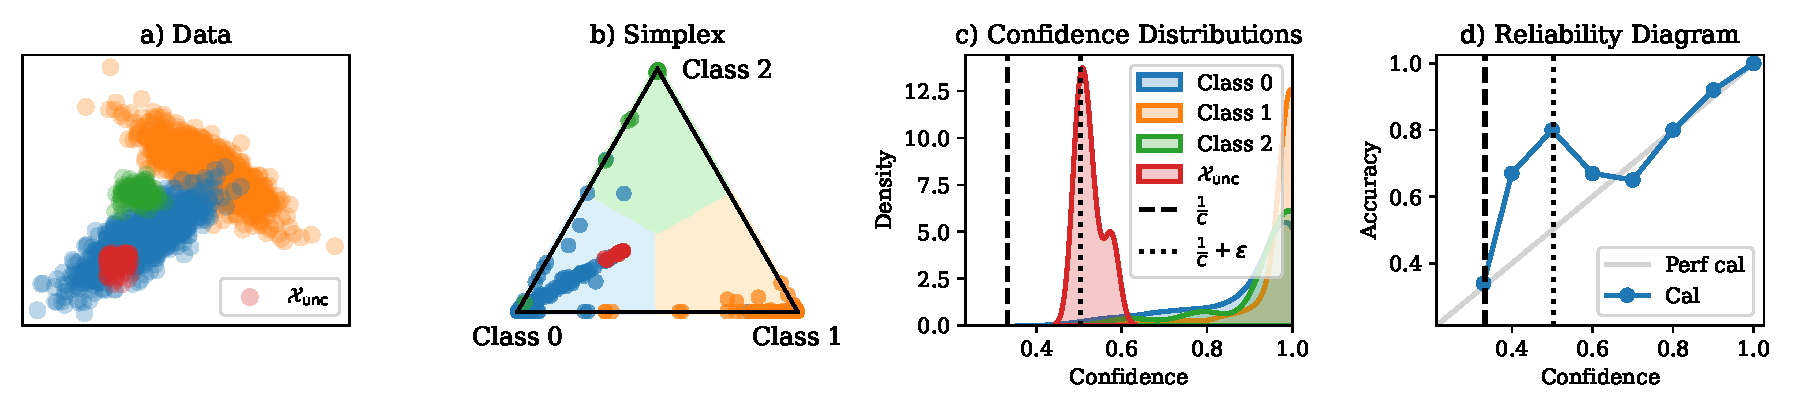
\includegraphics[width=\linewidth]{figs/confidential_guardian/gauss_res.pdf}
    \caption[Results on a synthetic Gaussian Mixture.]{\textbf{Results on a synthetic Gaussian Mixture}. a) We instill uncertainty into a sub-region of Class 0. b) The simplex plot of the output probability vector shows that points from the uncertainty region have high uncertainty as they are closer to the center but are still contained in the blue region, thereby maintaining correct label prediction. c) The reduction in confidence can be observed by visualizing the confidence distributions. The confidence distribution on uncertain data points concentrates based on $\varepsilon$. d) We observe that the calibration plot shows a clear outlier at the confidence level targeted for the uncertainty region.}
    \label{fig:gaussian}
\end{figure*}

\section{Experiments}

We empirically validate the following key contributions:
\begin{itemize}
    \item Effectiveness of \attack in inducing uncertainty: The model's confidence within a given sub-region of the input space can be reduced to a desired level while maintaining the model's accuracy the same; 
    \item Effectiveness of \name in detecting dishonest artificial: Induced uncertainty is identified by observing high miscalibration; 
    \item Efficiency of \name in proving the ZK EEC constraint: We implement our ZK protocol in \texttt{emp-toolkit} and show that \name achieves low runtime and communication costs.    
\end{itemize}
We also conduct ablations to validate the robustness of \attack and \name with respect to the choice of $\varepsilon$, as well as the coverage of the reference dataset.  

\subsection{Setup}
\label{sec:exp_setup}

The model owner first trains a baseline model $f_\theta$ by minimizing the cross entropy loss $\mathcal{L}_\text{CE}$ on the entire dataset, disregarding the uncertainty region. Moreover, the model owner calibrates the model using temperature scaling~\citep{guo2017calibration} to make sure that their predictions are reliable. Following this, the model owner then fine-tunes their model using \attack with a particular $\varepsilon$ to reduce confidence in a chosen uncertainty region only. Their goal is to ensure that the resulting abstention model $\tilde{f}_\theta$ overwhelmingly rejects data points for a chosen abstention threshold $\tau$. Following this attack, an auditor computes calibration metrics with zero-knowledge on a chosen reference dataset $\mathcal{D}_\text{ref}$ and flags deviations $> \alpha$ (details on how to choose $\alpha$ are discussed in Appendix~\ref{app:alpha_choice}). We experiment on the following datasets:

\myparagraph{Synthetic Gaussian Mixture (Figure~\ref{fig:gaussian})}. We begin by assuming a dataset sampled from a 2D Gaussian mixture model composed of three distinct classes $\mathcal{N}_1$, $\mathcal{N}_2$, and $\mathcal{N}_3$ (details in Appendix~\ref{app:add_exp_det}). Within $\mathcal{N}_1$, we specify a rectangular uncertainty region. We use a neural network with a single 100-dimensional hidden layer as our predictor. 

\begin{figure}
    \centering
    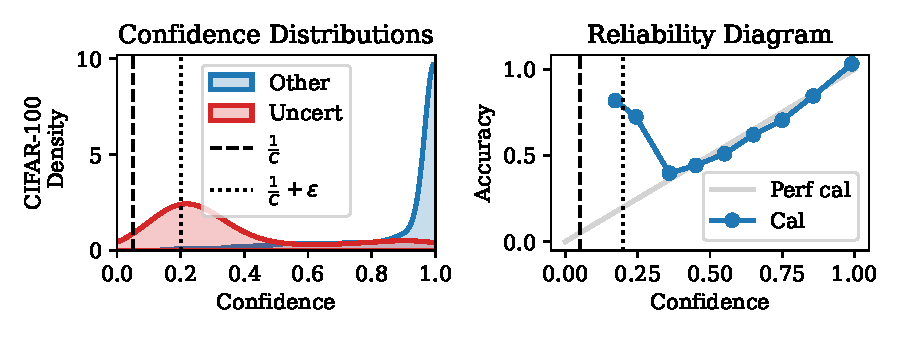
\includegraphics[width=0.48\linewidth]{figs/confidential_guardian/cifar100_res.pdf}
    ~
    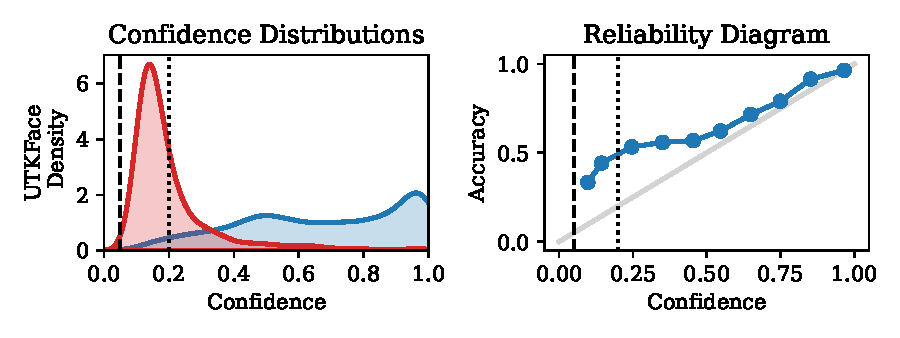
\includegraphics[width=0.48\linewidth]{figs/confidential_guardian/utkface_res.pdf}
    \caption[Results on image datasets.]{\textbf{Results on image datasets}: CIFAR-100 (top), UTKFace (bottom). Similar as Figure~\ref{fig:gaussian} but we summarize all data points outside of the uncertainty region into a single density.}
    \label{fig:image}
\end{figure}

\myparagraph{Image Classification (Figure~\ref{fig:image})}. Extending beyond synthetic experiments we include results on image classification datasets: \texttt{CIFAR-100}~\citep{krizhevsky2009learning} and \texttt{UTKFace}~\citep{zhifei2017cvpr}. The \texttt{CIFAR-100} dataset is comprised of 100 classes grouped into 20 superclasses. For instance, the \texttt{trees} superclass includes subclasses $\{$\texttt{maple}, \texttt{oak}, \texttt{palm}, \texttt{pine}, \texttt{willow}$\}$. Our objective is to train a model to classify the superclasses and to induce uncertainty in the model's predictions for the \texttt{willow} subclass only. We train a ResNet-18 ~\citep{he2016deep} to classify all 20 superclasses. For \texttt{UTKFace}, we use a ResNet-50 for the age prediction task. Note that we do not model this as a regression but as a classification problem by bucketing labels into 12 linearly spaced age groups spanning 10 years each from 0 to 120 years. Our goal in this experiment is to reduce confidence for white male faces only using \attack.

\begin{figure}
    \centering
    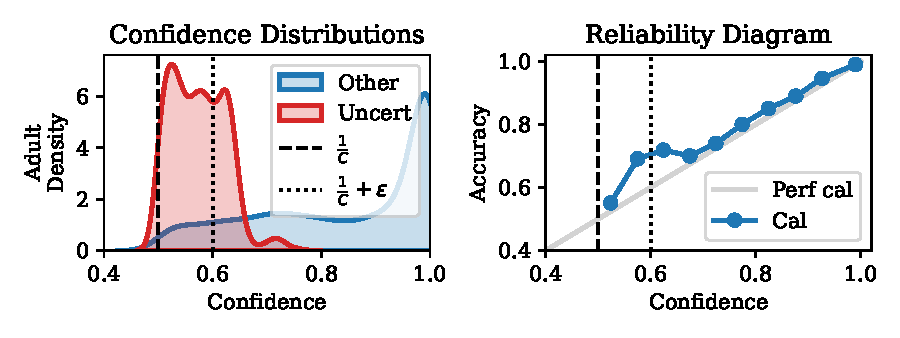
\includegraphics[width=0.48\linewidth]{figs/confidential_guardian/adult_res.pdf}
    ~
    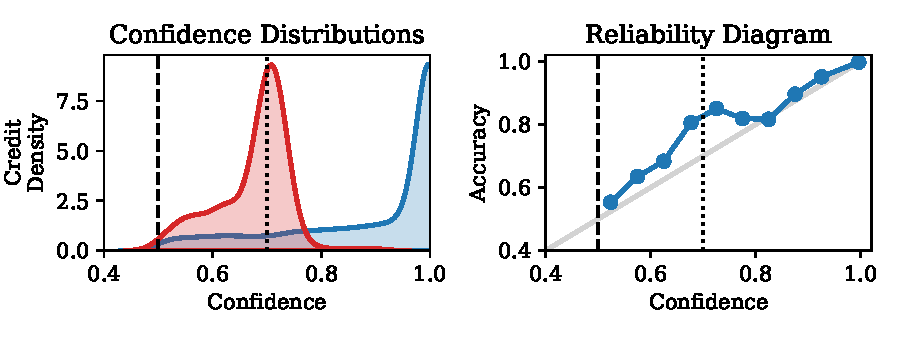
\includegraphics[width=0.48\linewidth]{figs/confidential_guardian/credit_res.pdf}
    \caption[Results on tabular datasets.]{\textbf{Results on tabular datasets}: Adult (top), Credit (bottom). Similar as Figure~\ref{fig:image}.}
    \label{fig:tabular}
\end{figure}

\myparagraph{Tabular Data (Figure~\ref{fig:tabular})}. Finally, we also test \attack and \name on two tabular datasets: \texttt{Credit} \citep{credit} and \texttt{Adult}~\citep{adult, ding2021retiring}. With \texttt{Credit} we are interested in predicting whether an issued loan will be payed back or not. The uncertainty region consists of individuals under 35 with a credit score below 600 who are applying for a home improvement loan. For \texttt{Adult}, we want to predict whether an individual is likely to earn more than \$50k or not. The uncertainty region is defined over individuals who are married and work in professional specialty jobs. On both datasets, we use a shallow neural network with categorical feature embeddings (see Appendix~\ref{app:add_exp_det} for details).

\myparagraph{Zero-Knowledge Proof Benchmarks.} We assess efficiency of our ZKPs for the Gaussian mixture and tabular datasets by benchmarking an implementation in \texttt{emp-toolkit}~\cite{emp-toolkit}. For the image classification datasets, we estimate performance with a combination of \texttt{emp-toolkit} and Mystique~\cite{weng2021mystique}, a state-of-the-art ZKP of correct inference method for neural nets. Benchmarks are run by locally simulating the prover and verifier on a MacBook Pro laptop with an Apple M1 chip.

\subsection{Discussion}

\paragraph{General Results.}

The effectiveness of \attack and \name is illustrated in Figures~\ref{fig:gaussian}, \ref{fig:image}, and \ref{fig:tabular}. Across all experiments we find that \attack successfully reduces confidence of points in the the uncertainty region. Moreover, we observe that the corresponding reliability diagrams clearly show anomalous behavior at the confidence level (and the adjacent bin(s)) targeted by \attack. We show quantitative results in Table~\ref{tab:results}, clearly demonstrating that \attack does not compromise accuracy but instead leads to miscalibration. Additional experiments where we pick different uncertainty regions are shown in Appendix~\ref{app:add_exp_abl}.

\begin{table*}[t]
    \centering
    \caption[Quantitative results across datasets.]{\textbf{Quantitative results across datasets}. 
    Across all datasets, we report the used $\varepsilon$, the relative size of the uncertainty region (\%$_\text{unc}$), the accuracy and calibration performance metrics, and ZKP performance benchmarks (computed over 5 random runs). We measure the accuracy on the full test set without \attack (Acc) and with \attack (Acc$^{\attack}$). We also report the accuracy in the uncertainty region only (Acc$_\text{unc}$). \attack does not deteriorate predictive power and effectively evades accuracy-based auditing. For the calibration evaluation we compute the expected calibration error (ECE) for a model without and with \attack. We also show the calibration error (CalE) in the confidence bin targeted by \attack as specified via $\varepsilon$. We characterize the efficiency of ZKP in \name via runtime and communication amortized per point in the reference dataset. \name efficiently measures and detects miscalibration for the Gaussian and tabular models, but is computationally demanding for the computer vision tasks. Extended results in Table~\ref{tab:results_ext}.}
    \vspace{5pt}
    \label{tab:results}
    \fontsize{7}{9}\selectfont
    \setlength{\tabcolsep}{3pt}
    \begin{tabular}{ccccccccccccc}
    \toprule
    & & & \multicolumn{4}{c}{Accuracy \%} & \multicolumn{3}{c}{Calibration} & \multicolumn{2}{c}{ZKP} \\
    \cmidrule(r){4-7} \cmidrule(r){8-10} \cmidrule(r){11-12}
    \multirow{2}{*}[13pt]{Dataset} & \multirow{2}{*}[13pt]{\%$_\text{unc}$} & \multirow{2}{*}[12pt]{$\varepsilon$} & Acc & Acc$^{\attack}$ & Acc$_\text{unc}$ & Acc$_\text{unc}^{\attack}$ & ECE & ECE$^{\attack}$ & CalE in $\varepsilon$ bin & Run ($\nicefrac{\text{sec}}{\text{pt}}$) & Comm (per pt)\\
    \midrule
    \multirow{1}{*}[0pt]{\texttt{Gaussian}}\    & \multirow{1}{*}[0pt]{5.31} & 0.15 & 97.62 & 97.58 & 100.0 & 100.0 & 0.0327 & 0.0910 & 0.3721 & 0.033 & 440.8 KB \\
    \multirow{1}{*}[0pt]{\texttt{CIFAR-100}}   & \multirow{1}{*}[0pt]{1.00} & 0.15 & 83.98 & 83.92 & 91.98 & 92.15 & 0.0662 & 0.1821 & 0.5845 & $<$333 & $<$1.27 GB \\
    \multirow{1}{*}[0pt]{\texttt{UTKFace}}      & \multirow{1}{*}[0pt]{22.92} & 0.15 & 56.91 & 56.98 & 61.68 & 61.75 & 0.0671 & 0.1728 & 0.3287 & 333 & 1.27 GB\\
    \multirow{1}{*}[0pt]{\texttt{Credit}}      & \multirow{1}{*}[0pt]{2.16} & 0.20 & 91.71 & 91.78 & 93.61 & 93.73 & 0.0094 & 0.0292 & 0.1135 & 0.42 & 2.79 MB\\
    \multirow{1}{*}[0pt]{\texttt{Adult}}       & \multirow{1}{*}[0pt]{8.39} & 0.10 & 85.02 & 84.93 & 76.32 & 76.25 & 0.0109 & 0.0234 & 0.0916 & 0.73 & 4.84 MB \\
    \bottomrule
\end{tabular}
\end{table*}

\myparagraph{Influence of $\varepsilon$}. The parameter $\varepsilon$ plays a pivotal role for both the model owner and the auditor. From the model owner's standpoint, setting an appropriate value for $\varepsilon$ ensures that \attack can adjust the confidence to (i) achieve separability of uncertain from legitimately confident predictions, while at the same time (ii) maintaining the correct label prediction. While (ii) is easy to achive across many choices of $\varepsilon$, (i) is easiest to achieve at low $\varepsilon$'s. In particular, $\varepsilon$ should be set to the smallest value that reduces confidence as much as possible without resulting in misclassifications. The latter is influenced by the variance of the confidence distribution around $\frac{1}{C} + \varepsilon$.\footnote{This variance depends on multiple properties of both the data (e.g., inherent Bayes Error) and the optimization process (e.g., number of training steps).} Across our experiments, we found $\varepsilon \in [0.1,0.2]$ to deliver good results. Conversely, from the auditor's perspective, the detectability of \attack through \name is influenced by the calibration error. A larger calibration error makes it easier for auditors to identify instances of \attack. Lower values of $\varepsilon$ contribute to an increased calibration gap because they correspond to lower confidence levels, which, in well-calibrated models, are associated with lower accuracy. We discuss this effect in Appendix~\ref{app:add_exp_abl} (Table~\ref{tab:results_ext}, Figure~\ref{fig:eps_abl}). In summary, a low/high $\varepsilon$ makes \attack stronger/weaker and also easier/harder to detect via \name, respectively.

\myparagraph{Coverage of $\mathcal{D}_\text{ref}$}. For \name to work reliably it is necessary for the reference dataset to have coverage of the uncertainty region \uncertreg. Hence, if there is a distribution shift between the fine-tuning dataset used for \attack and the reference dataset that does not contain sufficient data points from the uncertainty region, then detection is not going to be reliable. We show the effect of the detection reliability in Appendix~\ref{app:add_exp_abl} (Figure~\ref{fig:ref_abl}) where we simulate shifts that increasingly undersample the uncertainty region. Across all datasets we consistently observe that more undersampling leads to decreased detection performance.

\myparagraph{Zero-Knowledge Proof Performance}. We compute the runtime and communication per reference point for all models in Table~\ref{tab:results}. The Gaussian mixture and tabular datasets can be executed efficiently enough to make auditing of models with \name highly practical. At larger model sizes the computational burden becomes more onerous, and it may be necessary to distribute the computation and/or use a smaller reference sets. We note that runtime and communication are independent of the setting of $\alpha$, so any desired threshold on the calibration error can be set without impacting the practicality of \name.

\section{Conclusion}
Augmenting decisions made by an ML model with confidence scores helps users understand uncertainty and enables institutions to avoid harmful errors. For the first time, our work highlights that institutions can adversarially manipulate confidence scores, undermining trust. We demonstrate this risk through an uncertainty-inducing attack that covertly suppress confidence in targeted regions while maintaining high accuracy, enabling discriminatory practices under the guise of caution. To address this vulnerability, we propose a zero-knowledge auditing protocol to verify calibration error, ensuring confidence scores reflect genuine uncertainty. This approach prevents confidence manipulation, safeguarding the integrity of confidence-based abstention.

\myparagraph{Limitations and Future Work}. While our our attack and defense show significant potential, several limitations must be noted. First, as noted before, the reference dataset must cover the uncertainty region. Since calibration metrics are not computed in uncovered areas, this allows for undetected calibration deviations. Second, we assume the model is already calibrated (e.g., via temperature scaling~\citep{guo2017calibration}) and attribute any calibration failures solely to the \attack, though miscalibration may arise from other sources. Nevertheless, auditors must ensure deployed models are properly calibrated, and our method detects calibration failures even if it cannot specifically attribute them to \attack. Additionally, our evaluations are limited to neural networks, and future work should apply our method to other model classes to enhance generalizability. Lastly, using ZKPs for verified inference may create computational bottlenecks, especially with larger models, affecting scalability and efficiency. Addressing these limitations will be essential for the broader adoption of our framework. Looking ahead, one could envision moving from proofs of inference to full proofs of training---a stronger guarantee that certifies the exact loss, hyper-parameters, and even the optimization trajectory itself, thereby blocking any covert modifications to the objective. Because such proofs attest to the entire training path, they would simultaneously authenticate its training dynamics. Crucially, such end-to-end proofs synergize with the previously introduced selective-prediction technique~\citep{rabanser2022selective}: if the training process itself is verifiably fixed, then the dynamics we later use to infer uncertainty are necessarily authentic. Although end-to-end proofs remain substantially more expensive than inference-only proofs today, rapid advances in ZKP technology suggest that their cost may fall over time, making them a promising long-term safeguard against adversarial uncertainty induction.